\chapter{Konzeption und Entwurf}
\label{konzeption_und_entwurf}
In diesem Kapitel werden mögliche Probleme bei der Entwicklung sowie bei der Nutzung von JavaFX Anwendungen identifiziert. Dabei wird ein besonderer Fokus auf das Finden von Architekturmängeln, fehlenden Funktionalitäten und verbesserungswürdigen Techniken gelegt. Um eine Fehleranfälligkeit zu reduzieren, sollen komplexe und sich häufig wiederholende Quelltextbausteine automatisch erstellt oder durch Annotationen vereinfacht werden. Die vollständige Substitution eines aufwendigen Prozesses ist dabei ebenfalls möglich. Probleme, Vereinfachungen oder Verbesserungen sollen durch das Untersuchen von vorhandenen, quelloffenen JavaFX-Projekten und Bibliotheken gefunden werden. Auch sollen Ideen und Konzepte zusammengetragen werden, welche auf JavaFX anwendbar sind, jedoch nur in anderen Bibliotheken und Frameworks aufzufinden sind. \\
Bei der Problemanalyse wird stets das Ziel verfolgt, das Entwickeln mit JavaFX zu vereinfachen -- besonders für noch unerfahrene Entwickler. Danach wird eine Anforderungsanalyse durchgeführt, mit welcher systematisch funktionale sowie nichtfunktionale Anforderungen auf der Basis der gefundenen Probleme erstellt werden. \\
Auf die Anforderungserhebung folgt die Konzeption des benötigten Systems und der zugrundeliegenden Architektur. Essentielle Komponenten werden mit \ac{uml} Diagrammen entworfen und im Detail erläutert. Bei der Existenz verschiedener Lösungsstrategien für ein Problem, wird jede Strategie einzeln beleuchtet und nach Kriterien wie Sinnhaftigkeit und Machbarkeit entschieden, welche für das System am besten geeignet ist. Wichtige Richtlinien wie die angestrebte Softwarequalität werden ebenfalls beschrieben.

\section{Identifikation von Problemen und komplexen Strukturen in der JavaFX Entwicklung}
\sectionmark{Identifikation von Problemen}
\label{problemanalyse}
Im Folgenden werden generelle Probleme bei der Entwicklung von JavaFX Anwendungen identifiziert. Dazu gehören Mechanismen welche aufgrund ihrer Komplexität nicht für Anfänger geeignet sind oder von erfahrenen Entwicklern häufig genutzt und somit möglicherweise vereinfacht werden können. Obwohl dabei Annotationen als Basis für eine Vereinfachung dienen, wird auch das Erstellen von zusätzlichen Klassen oder dem Entwickeln von Erweiterungen für existierenden JavaFX Konzepte als Alternative für diese Zielerreichung in Betracht gezogen. Die Lösungen der gefundenen Probleme werden in einer Anforderungsanalyse durch funktionale und nichtfunktionale Anforderungen in \autoref{anforderungsanalyse} gelöst.
\subsection{Internationalisierung und Lokalisierung}
In der Informatik, speziell in der Softwareentwicklung, ist die Internationalisierung ein wichtiger Bestandteil einen Softwareproduktes, bei welchen die Entwickler die Software so gestalten, dass diese ohne viel Aufwand für andere internationale Märkte mit anderen Kulturen und Sprachen verfügbar gemacht werden kann \cite{Reineke2005}. Dabei wird beispielsweise eine einfache Schnittstelle für das Verwenden von verschiedenen Sprachen entwickelt, welche das Übersetzen von vorhandenen Textfeldern und anderen textbasierte Elementen in grafischen Benutzeroberflächen, Konfigurationsdateien oder Konsolenausgaben ermöglicht. Die Schnittstelle wird dabei so entwickelt, dass ohne eine Änderung des Quelltextes, neue Sprachen hinzugefügt werden können. Die Lokalisierung beschreibt dann unter Anderem die Übersetzung von den eben genannten Elementen.\\
Dieses Konzept kann durch die von Java bereitgestellte \texttt{ResourceBundle} Klasse realisiert werden \cite{Deitsch2001}. Bei der Verwendung eines solchen \texttt{ResourceBundle}s wird jedem zu übersetzenden Element ein Schlüssel zugeordnet und nach Konvention, in einer \texttt{.properties} Datei gespeichert. Wenn eine neue Sprache im Laufe des Lokalisierungsprozesses hinzugefügt werden soll, so muss jeweils eine neue \texttt{.properties} Datei angelegt werden. JavaFX ermöglicht das manuelle Spezifizieren einer vordefinierten \texttt{ResourceBundle} Instanz bei dem Laden einer FXML Datei durch einen \texttt{FXMLLoader}.
In der zu ladenden FXML Datei müssen hartcodierte Textelemente durch den jeweiligen Schlüssel aus der \texttt{.properties} Datei, wie in \autoref{lst:fxmlkey} gezeigt, ersetzt werden.
\begin{figure}[H]
	\noindent
	\begin{adjustbox}{minipage=[t]{.45\linewidth},gstore totalheight=\heightone,margin=\fboxsep+\fboxrule}
		\begin{lstlisting}
## Properties Datei
login.user = Benutzername
		\end{lstlisting}
	\end{adjustbox}\hfill
	\begin{adjustbox}{minipage=[t][\heightone]{0.5\linewidth}}
		\begin{lstlisting}[language=XML]
<!-- FXML Datei -->
<Label text="%login.username"/>
		\end{lstlisting}
	\end{adjustbox}
	\captionof{lstlisting}{Nutzung des Schlüssels in einer FXML Datei.}
	\label{lst:fxmlkey}
\end{figure}
\noindent Das Problem bei dieser Art der Übersetzung ist, dass eine Änderung der Sprache zur Laufzeit des Programms nicht dynamisch möglich ist. Die FXML Datei bzw. der dazugehörige Controller muss nach einer Sprachänderung durch beispielsweise eine Schaltfläche oder ein Dropdown-Menü durch einen FXML-Loader neu geladen werden, damit eventuelle Änderungen übernommen werden können. Das dynamische Ändern der Sprache zur Laufzeit ist nur mit einem Modifizierung des Ladeprozesses von FXML Dateien durch eine eigene Version des \texttt{FXMLLoader}s oder durch eine vom \texttt{FXMLLoader} unabhängige Implementierung durch Properties und Bindings möglich. Die erste Variante sorgt für ein automatisches Binden der nötigen Properties und die Letztere für ein manuelles Binden wenn nötig, weshalb eine Fusion beider Möglichkeiten in eine hohe Anpassbarkeit des Systems resultiert. Außerdem ist es auf diese Weise möglich, verschiedene Bindings zu aktualisieren, falls ein bestimmtes Event auftritt, welches eine Änderung des übersetzten Textes hervorruft. Parameterisierte Schlüssel aus der \texttt{.properties} Datei können somit automatisch an die parameterverändernden Events gebunden werden.
\subsection{Abhängigkeitsinjektion für Controller}
Bei der Abhängigkeitsinjektion werden Abhängigkeiten von Objekten zur Laufzeit des Programms bestimmt und zur Verfügung gestellt. Meist konfiguriert der Entwickler mithilfe einer externen Bibliothek die Bereitstellung der Abhängigkeiten in einer Konfigurationsdatei oder Konfigurationsklasse. Bei dem Nutzen einer Art von Abhängigkeitsinjektion ist die eigentliche Implementierung der Abhängigkeiten durch die abhängigen Objekte nicht bekannt. Diese kennen nur die Schnittstellen, weshalb ein Auswechseln der Schnittstellenimplementierung durch eine Änderung der jeweiligen Konfigurationsdatei/Konfigurationsklasse möglich ist. Durch diese explizite Trennung von Schnittstelle und Implementierung ist eine lose Kopplung der Komponenten gewährleistet, was wiederum zu einer hohen Flexibilität und zu einer hohen Wartbarkeit sowie Testbarkeit führt. Eine Injektion ist dabei durch Felder (Feldinjektion), Konstruktoren (Konstruktorinjektion) oder Setter (Setterinjektion) möglich. Die Funktionalität einer Injektion von Abhängigkeiten in einen Controller ist nicht direkt in JavaFX enthalten, kann aber durch das Verwenden von zum Beispiel Afterburner.fx\footref{ft:afterburner} hinzugefügt werden. Eine Unterstützung von etablierten externen Bibliotheken zur Realisierung des Abhängigkeitsinjektionsmusters wie Spring\footnote{Spring: \url{https://spring.io}}, Dagger\footnote{Dagger: \url{https://dagger.dev}} oder Guice\footnote{\label{ft:guice}Guice: \url{https://github.com/google/guice}} ist dadurch jedoch nicht gegeben. Aufgrund der Tatsache, dass alle drei genannten Bibliotheken mit der \texttt{jakarta.inject.Inject} Annotation\add{validate}, eine grundlegende Abhängigkeitsinjektion bereitstellen, kann ebendiese Annotation für eine Injektion innerhalb von Controllern verwendet werden. Ein Beispiel eines Controllers mit verschiedenen injizierten Diensten ist in \autoref{lst:controllerinjection} zu erkennen.
\begin{figure}[H]
	\centering
	\begin{lstlisting}[caption=Beispiel -- Controller mit injizierten Diensten., captionpos=b, label=lst:controllerinjection]
	public class TestController {
	
		#@Inject
		private IUserService userService;
		
		#@Inject
		private IDatabaseService dbService;
	
	}
	\end{lstlisting}
\end{figure}
\noindent Die Implementierungen sollen durch den Entwickler in der jeweiligen Konfigurationsdatei/Konfigurationsklasse den Schnittstellen zugeordnet werden können.
\subsection{CSS Metadatengeneration}
Ein wichtiger Bestandteil von JavaFX ist die Möglichkeit, das Aussehen und den Stil von einzelnen Komponenten wie Schaltflächen und Containerelementen durch die Verwendung von \ac{css} zu modifizieren. Werden eigene Komponenten erstellt oder bestehende Komponenten erweitert, so erlaubt JavaFX das Hinzufügen von eigenen \ac{css} Properties zu den jeweiligen Komponenten mithilfe von neuen Instanzen der \texttt{CssMetaData} Klasse. Für jede neue \ac{css} Property muss dabei eine neue \texttt{CssMetaData} Instanz erstellt werden, weshalb das Hinzufügen von vielen solcher Instanzen ein repetitiver Prozess mit vielen Boilerplate Quelltextfragmenten ist, welcher durchaus vereinfacht werden kann.
\subsection{JavaFX Einstiegspunkt und Preloader}
Damit eine JavaFX Applikation gestartet werden kann muss, wie in \autoref{javafx} beschrieben, 
eine Klasse existieren, welche von der \texttt{Application} Klasse erbt. Müssen bestimmte performanceintensive Aufgaben wie das Laden von Sound-/Video- oder Bilddateien vor dem Start der eigentlichen Anwendungen ausgeführt werden, so kann dies in einer Klasse, welche von der \texttt{Preloader} Klasse erben muss, realisiert werden. Der \texttt{Preloader} ist dabei eine spezialisierte Form der \texttt{Application}, welche es dem Entwickler ermöglicht, Ressourcen zu laden und durch eventbasierte Statusaktualisierungen, dem Nutzer mitzuteilen. Damit ein \texttt{Preloader} mit einer standardmäßigen JavaFX Anwendung verbunden werden kann, muss statt \texttt{Platform\#launch}, die interne \texttt{PlatformImpl\#launchApplication} Methode genutzt werden. Das Verwalten der Aufgaben, welche vor dem Anwendungsstart durchgeführt werden müssen, soll vereinfacht werden, wobei insbesondere die vorhandenen Statusaktualisierungen  erweitert werden sollen. Auch die Initialisierung einer Applikationsklasse bzw. der benötigten \texttt{Stage} läuft in den meisten Fällen gleich ab und soll bei Bedarf vom Entwickler zu einem großen Teil automatisiert werden können.
\subsection{Controller Lebenszyklus}
\label{controller_lebenszyklus}
Der Lebenszyklus von JavaFX Controllern ist in der aktuellen Ausführung für komplexe Systeme mit vielen Controllern ungeeignet, da dieser nur aus zwei Phasen besteht. Zuerst wird die Controllerklasse instanziiert und darauf folgt die Initialisierung der \texttt{@FXML} Felder und der Methodenaufruf einer vom Entwickler bereitgestellten \texttt{initialize} Methode. Damit mit fertig initialisierten \texttt{@FXML} Feldern gearbeitet werden kann, muss der dafür benötigte Quelltext immer in der \texttt{initialize} Methode definiert werden. Ein Beispiel für den Ablauf einer Controllerinstanziierung durch den \texttt{FXMLLoader} ist in \autoref{lst:controllerinstantiation} abgebildet. Der rudimentäre Lebenszyklus unterstützt dabei keine Methoden, welche beispielsweise bei einem Entfernen des Wurzelelements eines Controllers aus dem Szenengraphen ausgeführt wird um eventuell offene Ressourcen zu schließen und somit effektiv Ressourcenlecks zu verhindern. Ein vollständiger Lebenszyklus wie bei Activities in Android\footnote{\url{https://developer.android.com/guide/components/activities/activity-lifecycle}},ist praktisch nicht vorhanden.
\begin{figure}[H]
	\centering
	\begin{lstlisting}[caption=Beispiel -- Instanziierungsablauf., captionpos=b, label=lst:controllerinstantiation]
public class TestController {
	
	@FXML
	private Label testLbl;
	
	public TestController() {
		// Phase #1 - Controllerinstanziierung
		// testLbl-Feld ist hier noch nicht initialisiert
	}
	
	@FXML
	private void initialize() {
		// Phase #2 - Feldinjektion fertiggestellt
		// testLbl-Feld ist initialisiert und kann verwendet werden
	}
	
}
	\end{lstlisting}
\end{figure}
\subsection{Konfigurationsdateien}
Eine persistente Speicherung von Anwendungskonfigurationen wie beispielsweise Logindaten oder Informationen für Serververbindungen ist wichtig für eine optimale Benutzerfreundlichkeit. Das Speichern von konfigurierbaren Einstellungen kann mit der Java Preferences API oder mit externen Bibliotheken wie GSON, für auf \ac{json} basierte Konfigurationsdateien oder \ac{jaxb}, für auf \ac{xml} basierte Dateien durchgeführt werden. Der Prozess des manuellen Erstellens einer Konfigurationsdatei und dem anschließenden Auslesen bzw. Modifizierung zur Laufzeit ist ein repetitiver Vorgang, welcher durch das Nutzen von Annotationen teilweise automatisiert werden kann.
\subsection{Zustandsserialisierung von grafischen Oberflächen}
Das Speichern des aktuellen Zustands einer grafischen Oberfläche mit den jeweiligen Elementen ist aktuell mit dem Funktionsumfang von JavaFX nicht ohne Weiteres umsetzbar. Der Zustand einer Anwendung setzt sich aus den aktuellen Konfiguration von interaktiven Elementen im Szenengraphen zusammen. Beispielsweise ist die Position eines Schiebereglers oder der aktuell ausgewählte Tab einer \texttt{TabPane} nicht insoweit serialisierbar, dass dieser Zustand beim Applikationsende gespeichert und bei einem erneuten Applikationsstart wiederhergestellt werden kann.
\section{Anforderungsanalyse}
\label{anforderungsanalyse}
In der Anforderungsanalyse werden die gefundenen Problemlösungen und Vereinfachungen aus \autoref{problemanalyse} in Form von funktionalen und nichtfunktionalen Anforderungen formuliert. Dabei werden die Anforderungen in zwei Klassen unterteilt:
\begin{description}
	\item \textbf{Fundamentale Anforderungen} sind Anforderungen, welche für eine Funktion des Systems essentiell sind, alle genannten Probleme weitgehend beheben und daher zwangsläufig implementiert werden müssen. Alle folgenden fundamentalen Anforderungen haben den [+A--\#\#] Präfix, wobei + durch die Art der Anforderung (funktional, nichtfunktional) und \#\# durch die jeweilige Anforderungsnummer substituiert wird.
	\item \textbf{Optionale Anforderungen} sind Anforderungen, welche keinen Einfluss auf eine ordnungsgemäße Funktionalität des Systems haben. Sie sind optional und werden möglicherweise aufgrund ihrer Komplexität nur teilweise oder gar nicht implementiert und können stattdessen für eine Erweiterung des Systems durch weitere Entwickler genutzt werden. Alle folgenden optionalen Anforderungen haben den (+A--\#\#) Präfix, wobei + durch die Art der Anforderung (funktional, nichtfunktional) und \#\# durch die jeweilige Anforderungsnummer substituiert wird.
\end{description}

% counter for functional requirements
\newcounter{fcounter}
\setcounter{fcounter}{0}
\newcommand*{\freq}[1]{%
	\protecting{\stepcounter{fcounter}\ifblank{#1}{[FA--\ifnum\value{fcounter}<10 0\fi\arabic{fcounter}]}{(FA--\ifnum\value{fcounter}<10 0\fi\arabic{fcounter}) Optional --\label{freq\arabic{fcounter}}}}%
}

% counter for nonfunctional requirements
\newcounter{ncounter}
\setcounter{ncounter}{0}
\newcommand*{\nreq}[1]{%
	\protecting{\stepcounter{ncounter}\ifblank{#1}{[NFA--\ifnum\value{ncounter}<10 0\fi\arabic{ncounter}]}{(NFA--\ifnum\value{ncounter}<10 0\fi\arabic{ncounter}) Optional --}\label{nreq\arabic{ncounter}}}%
}

\subsection{Funktionale Anforderungen}
\label{anforderungsanalyse_funktional}

\renewcommand\thesubsubsection{KAT/%
	\ifnum\value{subsubsection}<100 0\fi
	\ifnum\value{subsubsection}<10 0\fi
	\arabic{subsubsection}}

Im Folgenden werden alle funktionalen Anforderungen definiert. Sie beschreiben alle gewünschten Funktionen des Endproduktes.
\subsubsection{\freq{} Ermitteln und Konfiguration des JavaFX-Einstiegspunktes}
Der Erstellen einer Applikationsklasse sowie eines optionalen Preloaders soll automatisch stattfinden, da der Erstellungsprozess von auf JavaFX basierten Anwendungen in den meisten Fällen ähnlich oder identisch ist. Das Definieren dieser Elemente soll mithilfe von Annotationen geschehen und durch das Absuchen des Klassenpfades durch die entwickelte Bibliothek gefunden werden. Alternativ soll der Entwickler die Möglichkeit haben, den Einstiegspunkt sowie den Preloader explizit zu spezifizieren, falls eine automatische Identifikation nicht erwünscht oder benötigt ist. Die vordefinierten Einstiegspunkte sollen eine Standardkonfiguration der Applikation und der zugrunde liegenden \texttt{Stage} Instanz bereitstellen, welche durch den Entwickler bei Bedarf auch manuell überschrieben werden kann. Dieses Überschreiben soll durch die Nutzung des Erbauer-Entwurfsmusters oder durch Annotationen erfolgen. Die Standardkonfiguration umfasst grundsätzliche Applikationseigenschaften wie den Titel, die Fenstergröße oder Designelemente wie den \texttt{StageStyle} und die benötigten Titelleistenschaltflächen.
\subsubsection{\freq{} Eventbasierte Verwaltung des Applikationslebenszyklus}
Die Verwaltung des Applikationslebenszyklus soll mithilfe von Annotationen im Einstiegspunkt geschehen. Der Applikationslebenszyklus bezeichnet hier die vererbbaren \texttt{Application\#init}, \texttt{Application\#start} und \texttt{Application\#stop} Methoden. Die Erstellung der Applikationsklasse soll wie in \autoref{TODO} beschrieben, durch die zu entwickelnde Bibliothek übernommen werden, weshalb die Aufrufe der eben genannten Methoden durch ein Event-System an den vom Entwickler spezifizierten Einstiegspunkt delegiert werden sollen. Beispielsweise wird statt der Überschreibung der \texttt{Application\#start} Methode, eine Methode im Einstiegspunkt definiert, welche ein \texttt{StartEvent} als Parameter erhält und eine spezielle Annotation aufweist. Methoden für einen optionalen Preloader, sollen analog dazu definiert werden können.
\add{Maybe add}
%\subsubsection{\freq{} Vordefinierte Preloader-Zustandsänderungsbenachrichtigungen}
\subsubsection{\freq{} Dynamische Laufzeitübersetzung von JavaFX-Komponenten}
Die bereits existierenden Internationalisierungsmöglichkeiten sollen durch eine dynamische Übersetzung erweitert werden. Das Ändern der aktuellen Sprache soll durch beispielsweise einen Schaltflächenklick ausgelöst werden und zur Laufzeit die grafische Benutzeroberfläche aktualisieren. Ein Neustart der Anwendung oder ein erneutes Laden der FXML Dateien soll nicht mehr nötig sein. Der Entwickler soll dabei JavaFX Komponenten in Form von Objektattributen in Controllern annotieren können, welche durch eine verbesserte Version der \texttt{FXMLLoader} Klasse geladen und instanziiert werden sollen. Das dynamische Übersetzen der in der FXML Datei definierten Elemente soll per Element deaktivierbar sein. Die Funktionalität von externen FXML Parsern wie den Scene-Builder soll durch das Hinzufügen von eigener FXML Syntax dabei nicht kompromittiert werden. Übersetzbare Elemente, welche auf parameterabhängigen Übersetzungsschlüsseln basieren, sollen an JavaFX Properties gebunden werden können und bei Änderung dieser aktualisiert werden. Wird eine dynamische Übersetzung für nicht annotierbare Prozesse wie das Ausgeben von Nachrichten auf der Konsole oder generelle methodeninterne Textverarbeitung benötigt, so soll der Entwickler auf Utility-Klassen der Bibliothek zurückgreifen können, welche ebendiese Funktionalität zur Verfügung stellen.
\subsubsection{\freq{} Abhängigkeitsinjektion durch etablierte externe Bibliotheken}
Werden externe Bibliotheken zur Abhängigkeitsinjektion genutzt, so sollen eventuelle Abhängigkeiten und Dienste automatisch in Controller injiziert werden. Die Nutzung etwaiger Bibliotheken und den dafür benötigten Konfigurationsdateien oder Konfigurationsklassen soll beim Start der Applikation spezifiziert werden können. Eine Unterstützung der Bibliotheken Dagger, Spring und Guice soll dem Entwickler ermöglicht werden.
\subsubsection{\freq{} Automatische \ac{css} Metadaten Generation}
Das Hinzufügen von \ac{css} Properties zu benutzerdefinierten JavaFX Komponenten durch den Entwickler soll durch das Nutzen von Annotationen erleichtert werden. Durch die automatische Generation dieser Metadaten, sollen eventuell auftretende repetitive Quelltextbausteine vermieden werden. Das Initialisieren der JavaFX Anwendung durch die zu entwickelnde Bibliothek soll in eine Durchsuchung des Klassenpfades nach solchen \ac{css} Metadaten Annotationen resultieren und die gefundenen Metadaten automatisch mit den durch die Annotation definierten Einstellungen instanziieren.
\subsubsection{\freq{} Annotationsbasierte Controllerdefinition}
Ein Controller soll als solcher erkannt werden, wenn dieser eine spezielle Annotation aufweist. Die Annotation muss dabei die Quelle der FXML und der \ac{css} Datei enthalten und weitere auf Controller bezogene Konfigurationsmöglichkeiten bereitstellen.
\subsubsection{\freq{} Erweiterung des Controllerlebenszyklus}
Der Lebenszyklus eines Controllers soll, ähnlich wie bei Android Activities, in mehrere Phasen eingeteilt sein, welche durch die Nutzung von Annotationen durch den Entwickler abrufbar gemacht werden sollen. Methoden, welche nach einer bestimmten Phase ausgeführt werden sollen, sollen mit der zu der Phase gehörenden Annotation annotiert werden können. Der Lebenszyklus soll um folgende Phasen erweitert werden:
\begin{itemize}
	\item In der \textbf{\texttt{AfterInject}} Phase sind alle Abhängigkeitsinjektionen und alle Instanziierungen von JavaFX Komponenten vollständig abgeschlossen und somit durch den Entwickler im Controller verwendbar.
	\item In der \textbf{\texttt{OnShow}} Phase wird das Wurzelelement des Controllers im Szenengraphen aktiv gerendert und ist somit durch den Endbenutzer in der grafischen Benutzeroberfläche zu erkennen.
	\item In der \textbf{\texttt{OnHide}} Phase wurde das Wurzelelement des Controllers aus dem Szenengraphen entfernt und dementsprechend nicht gerendert.
	\item In der \textbf{\texttt{OnDestroy}} Phase werden alle zwischengespeicherten Ressourcen und Informationen des Controllers entfernt. In dieser Phase sollen eventuell offene Ressourcen geschlossen werden. Damit der Controller wiederverwendet werden kann, muss eine erneute Initialisierung durch beispielsweise einen \texttt{FXMLLoader} erfolgen.
\end{itemize}
\subsubsection{\freq{} Unterstützung von mehreren Lebenszyklusbehandlungsmethoden}
Wenn mehrere Methoden mit denselben Lebenszyklusannotationen annotiert wurden, so soll die Reihenfolge der Aufrufe dieser, anhand eines optionalen Parameters in der Annotation bestimmt werden. Weisen mehrere Annotationen dieselbe Priorisierung auf, so soll nach der Deklarationsreihenfolge in der Klasse sortiert werden.
\subsubsection{\freq{} Controllerverschachtelung und Supercontroller}
Ist das Wurzelelement eines Controllers in einem durch einen weiteren Controller aufgespannten Teilbaum des Szenengraphen enthalten, so handelt es sich bei ersterem Controller um einen Subcontroller des Letzteren. Subcontroller sollen bei Phasenänderung des Lebenszyklus ihres Supercontrollers benachrichtigt werden. Beispielsweise soll der Subcontroller in die \texttt{OnHide} Zustand wechseln, wenn der Supercontroller in denselben Zustand wechselt. Diese Beziehung soll bei Möglichkeit automatisch ermittelt werden aber dennoch explizit durch den Entwickler bei der Controllerdefinition deklariert werden können.
\subsubsection{\freq{} Gruppierung von ähnlichen Controllern}
Ähnliche Controller sollen bei Definition, sogenannten Controllergruppen zugeordnet werden können. Eine Controllergruppe teilt sich dasselbe Wurzelelement, weshalb immer nur ein Controller einer Controllergruppe gleichzeitig aktiv sein kann. Ein Controller soll dabei nur einer Controllergruppe zuordenbar sein. Wechselt der aktive Controller einer Controllergruppe, so soll die Controllergruppe davon in Kenntnis gesetzt werden und eventuelle Phasenwechsel von betroffenen Controllern ausgelöst werden. Verschachtelte Subcontroller sollen dabei zwischen einem Wechsel durch einen Supercontroller und einem selbst ausgelösten Wechsel differenzieren können.
\subsubsection{\freq{} Zyklusprävention}
Damit keine unendlichen Schleifen und Prozesse aus dem falsche Nutzen des Systems resultieren, muss eine Art von Zyklusdetektion bei der Verschachtelung von Controllern erfolgen. Beispielsweise darf Controller A nicht als Supercontroller von Controller B definiert sein, wenn B, den Controller A ebenfalls als Supercontroller definiert.
\subsubsection{\freq{} Wechsel von Controllern}
Das Wechseln von Controllern soll durch das vom Controller-System bereitgestellte Eventsystem ermöglicht werden. Ein manuelles Wechseln der Controller soll somit durch die Absendung eines Events durchführbar sein. Das automatische Wechseln eines Controllers soll durch vereinfachende Strukturen wie Annotationen über Schaltflächendefinitionen erleichtert werden. Der Entwickler soll den Wechsel durch die Angabe von Animationsparametern ästhetisch individualisieren können.
\subsubsection{\freq{} Controller Preloading}
Controller werden standardmäßig On-Demand geladen, also nur dann, wenn sie benötigt werden. Wenn der Entwickler einen Preloader definiert hat, dann soll das Erstellen und Initialisieren aller controllerrelevanten Elemente und Strukturen in dieser Preloading-Phase stattfinden können.
\subsubsection{\freq{} Globale Fehlerbehandlung}
Beim Start der Anwendung, sollen optionale Klassen zur globalen Fehlerbehandlung spezifiziert werden können. Wird eine solche Klasse nicht durch den Entwickler angegeben, so soll auf eine vom System bereitgestellte Klasse zur Fehlerbehandlung zurückgegriffen werden. Auftretende Fehler im Controllersystem, ob reflektiv bedingt oder nicht, sollen so an zentraler Stelle verwaltet und optional als Fehleranzeige auf dem Hauptcontroller angezeigt werden können.
\subsubsection{\freq{} Geteilte Ressourcen}
Controller sollen die Möglichkeit haben, bestimmte Felder mit anderen Controllern zu teilen. Geteilte Felder werden als solche identifiziert, wenn diese eine spezielle Annotation aufweisen. Das Controller-System soll dabei Referenzen von den jeweiligen Feldwerten erstellen und diese dann in Form von JavaFX Properties zur Verfügung zu stellen. Geteilte Ressourcen sollen dabei durch ihren Feldnamen oder optional durch einen Parameter der Annotation identifiziert werden. Der Annotationsparameter hat dabei immer eine höhere Priorität. Wird der Wert einer geteilten Ressource geändert, so soll sich diese Änderung in allen anderen Controllern mit ebendieser Ressource widerspiegeln.
\subsubsection{\freq{} JavaFX Events durch Annotationen}
Häufig genutzte JavaFX Events wie beispielsweise das \texttt{ActionEvent} sollen durch einfache Annotationen mit im Controller definierten Methoden assoziiert werden. Tritt ein über diese Methode definiertes Event auf, so soll die dazugehörige Methode des Controllers aufgerufen werden. Damit die Verbindung zwischen Feld und Methode gewährleistet ist, müssen beide Elemente annotiert werden und einen gemeinsamen Identifikator, welche den Annotationen als Parameter übergeben wird, aufweisen.
\subsubsection{\freq{} Generation von Konfigurationsdateien}
Felder eines Controllers sollen bei der Controllererstellung, durch das Nutzen von automatisch oder manuell erstellten Konfigurationsdateien, gesetzt werden, falls diese eine spezielle Annotation aufweisen. Der Konfigurationsschlüssel kann durch einen Annotationsparameter festgelegt werden.
\subsubsection{\freq{o} Serialisierung von JavaFX Komponenten}
Die Position und die aktuelle Konfiguration von jedem JavaFX Element, welches im Szenengraphen präsent ist, soll bei einem Ende der Anwendung gespeichert werden und bei dem nächsten Start rekonstruiert werden. Dadurch bleibt der aktuelle Zustand der grafischen Oberfläche auch bei Anwendungsterminierung erhalten.
\subsubsection{\freq{o} Scheduling von Methoden}
Controllerinterne Methoden sollen von Entwickler als sog. Scheduler definiert werden. Eine solche Methode wird dann in einem bestimmten Zeitintervall automatisch ausgeführt und gegebenenfalls wiederholt. Das Verhalten der Methode (wiederholend, zeitverzögert) kann durch Annotationsparameter kontrolliert werden.
\subsubsection{\freq{o} JavaFX Application-Thread Forcierung}
Einige Operationen auf Elemente des JavaFX Szenengraphen müssen auf dem JavaFX Application-Thread ausgeführt werden. Dazu gehört beispielsweise das aktive Ändern von renderbaren Elementen wie Textfeldinhalte oder Schaltflächen. Controllerinterne Methoden sollen auf dem JavaFX Application-Thread ausgeführt werden, wenn diese eine bestimmte Annotation aufweisen.
\subsubsection{\freq{o} Annotationsvalidierung zur Kompilierzeit}
Reflektive Operationen sind definitionsbedingt nur per Laufzeit der Anwendung ausführbar. Das Auslesen und Verarbeiten von annotierten Elementen und Annotationen im Allgemeinen durch reflektive Operationen kann somit nur zur Laufzeit erfolgen. Ob eine Annotation inkorrekte oder ungenügende Informationen enthält oder falsche Typen annotiert wurden ist dem Entwickler nur durch die Auslösung von Ausnahmen zur Laufzeit mitzuteilen. Beispielsweise ist es offensichtlich inkorrekt, ein Feld, welches einen JavaFX Container repräsentiert (z.B. \texttt{StackPane}), mit einer Annotation zu annotieren, welche für die Übersetzung von Komponenten verantwortlich ist. Das Überprüfen der Korrektheit der Annotationsnutzung soll nicht nur durch eine Laufzeitfehlerbehandlung sondern auch durch einen Annotationsprozessor zur Kompilierzeit durchgeführt werden. Eventuelle Fehlkonfigurationen werden somit bereits beim Kompiliervorgang entdeckt und dem Entwickler mitgeteilt.

\subsection{Nichtfunktionale Anforderungen}
\label{anforderungsanalyse_nichtfunktional}
Im Folgenden werden alle nichtfunktionalen Anforderungen definiert. Sie beschreiben Qualitätseigenschaften an das System wie Möglichkeiten der Erweiterbarkeit und Wartbarkeit und spezifizieren Maßstäbe, welche zur Laufzeit der Anwendung eingehalten werden müssen. Darunter gehören beispielsweise die effiziente Ressourcennutzung, die Korrektheit des Systems sowie ein gewisser Grad an Zuverlässigkeit.
\subsubsection{\nreq{} Benutzerfreundlichkeit}
Das Erstellen von JavaFX Anwendungen soll durch das Nutzen der zu entwickelnden Bibliothek erleichtert werden. Um diese Erleichterung sicherzustellen, müssen implementierte Komponenten ausreichend dokumentiert sein und intuitiv durch den Entwickler nutzbar gemacht werden. Komplexe und überflüssige Strukturen sollen vermieden werden. Jedes durch diese Bibliothek bereitgestellte konfigurierbare System, muss Standardparameter zur Konfiguration bereitstellen und bei Bedarf eine Konfigurationsänderung durch einen Entwickler zulassen.
\subsubsection{\nreq{} Performance \& Effizienz}
Obwohl das vollständige System an vielen Stellen die Reflection API nutzen muss, soll sowohl der Entwickler als auch der Endnutzer keinen gravierenden Performanceunterschied feststellen können. Es soll sichergestellt werden, dass der durch die Reflection API geschaffene Performanceoverhead, minimal gehalten wird.
\subsubsection{\nreq{} Wartbarkeit}
Die Bibliothek soll ohne viel Aufwand an sich verändernde Anforderungen anpassbar sein. Dazu muss das System allgemein anerkannte, softwaretechnische und objektorientierte Prinzipien erfüllen.
\subsubsection{\nreq{} Erweiterbarkeit}
Die Architektur soll mit einer besonderen Fokussierung auf das Nutzen von Schnittstellen entwickelt werden. Annotationsbasierte Konzepte, welche nicht im Standardumfang der von der Bibliothek bereitgestellten Funktionalitäten enthalten sind, sollen ohne viel Aufwand durch externe Entwickler hinzugefügt werden können.
\subsubsection{\nreq{} Softwarequalität}
Eine hohe Softwarequalität ist ein essentieller Faktor für ein System, welches auch außerhalb der eigenen Entwicklungsumgebung genutzt werden soll. Andere Entwickler müssen mit einem geringen Zeitaufwand, einen Überblick über das System mit allen wichtigen Komponenten und deren Beziehung untereinander, gewinnen können. Um eine hohe Nachvollziehbarkeit zu gewährleisten, müssen etablierte Entwurfsmuster genutzt und auf komplexen Quelltext verzichtet werden. Klassen müssen gut strukturiert und leicht verständlich implementiert werden.
\subsubsection{\nreq{} Lizenzierung}
Die zu entwickelnde Bibliothek muss eine Konformität zu den von externen Bibliotheken genutzten Lizenzen aufweisen. Etwaige Lizenzverletzungen sind zu vermeiden.

\section{Konzept und Modellierung}
\label{konzept_und_modellierung}
Im Folgenden wird die, für das Erfüllen aller vorher genannten Anforderungen, benötigte Architektur konstruiert. Dabei werden ähnliche Systemanforderungen in Gruppen unterteilt und in Form von allgemeinen Zielen an das System zusammengefasst. Für jedes daraus resultierende Ziel, werden theoretische Implementierungsmöglichkeiten identifiziert, bei welchen benötigte Komponenten, die Beziehung zwischen den Komponenten und die eventuelle Nutzung von Entwurfsmuster ermittelt werden. Dabei wird besonders auf eine hochwertige Softwarequalität und Usability geachtet. Grundlegende, notwendige Entscheidungen wie die Namensgebung der Bibliothek und die Nutzung von externen Bibliotheken für eine effizientere und leichtere Implementierung werden ebenfalls getroffen. 
\subsection{Ziele des Systems}
Aus der Problemanalyse und der nachfolgenden Erhebung von funktionalen und nichtfunktionalen Anforderungen ergeben sich drei grundlegende Ziele des Systems:
\begin{itemize}
	\item Erstellung von auf Annotationen basierenden Vereinfachungen für anspruchsvolle Aspekte der JavaFX-Programmierung.
	\item Erweiterung von bereits existierenden Funktionen wie die Lokalisierung und die Controllerverwaltung.
	\item Hinzufügen von Funktionen, welche aktuell nicht im Funktionsumfang von JavaFX enthalten sind wie die Abhängigkeitsinjektion.
\end{itemize}
Alle Ziele sollen neuen Entwicklern den Einstieg in JavaFX erleichtern aber auch erfahrenen Entwicklern die Möglichkeit geben, effizienter mit JavaFX zu programmieren. Dazu müssen diese nicht unbedingt die vom System zu Verfügung gestellten Annotationen verwenden, sondern können auch die Utility Klassen und eventuell die vereinfachte Schnittstelle zur Java Reflection API nutzen.
\subsection{Rahmenbedingungen und Designentscheidungen}
\label{konzept_und_modellierung_designentscheidungen}
Nachfolgend werden grundlegende Designentscheidungen der Softwarearchitektur und Rahmenbedingungen für die Entwicklung der Software als Ganzes dargelegt.
\subsubsection{Namensgebung}
Die zu entwickelnde Bibliothek benötigt einen Namen, welcher die Beziehung zu JavaFX verdeutlicht und gleichzeitig aufzeigt, dass die Vereinfachung und die Erweiterung von JavaFX Bausteinen und einzelnen Komponenten angestrebt wird und deshalb die oberste Priorität darstellt. Nachfolgend wird die Bibliothek als \textbf{\texttt{SimpliFX}} bezeichnet. \texttt{SimpliFX} ist dabei an das englische Wort \texttt{simplify} angelehnt, welches ins Deutsche übersetzt \texttt{vereinfachen} bzw. \texttt{simplifizieren} bedeutet. Damit die Verbindung zu Java\texttt{FX} untermauert wird, ist das \texttt{FY} Suffix durch das \texttt{FX} Suffix substituiert worden.
\subsubsection{Modularisierung}
Gute Softwaresysteme bestehen aus vielen Komponenten, welche jeweils auf eine einzelne Funktion spezialisiert sind. Einige dieser Komponenten funktionieren unabhängig von Anderen und können durch eine Dekomposition des Systems in unterschiedliche Module unterteilt werden. Eine modulare Softwarearchitektur folgt dem softwaretechnischen \ac{soc} Prinzip und resultiert in einer hohen Wartbarkeit sowie Erweiterbarkeit. Außerdem ermöglicht eine Modularisierung, dass einzelne Module aufgrund ihrer strikten Trennung einfacher ausgetauscht werden können.\\
Häufig genutzte reflektive Operationen der Reflection API müssen durch eine einfache Schnittstelle für \texttt{SimpliFX} zugänglich gemacht werden. Diese Schnittstelle muss ein ordnungsgemäße Ausnahmebehandlung aufweisen, da das Nutzen der Reflection API sehr fehleranfällig ist und sehr effizient implementiert werden, da etwaige Operationen langsamer sind als Nutzen von herkömmlichen Java-Sprachfeatures. Diese Schnittstelle wird in einem von \texttt{SimpliFX} unabhängigen Apache Maven\footref{ft:maven} Modul ausgelagert. Auch die Testapplikationen, welche nach der Implementierung des eigentlichen Systems entwickelt werden und für die Evaluation von diesem dienen, werden in ein anderes Modul ausgelagert. Das Basissystem ist somit in einem dritten Modul zu finden und ist für die aus den Systemanforderungen resultierenden Funktionalitäten verantwortlich. Die verschiedenen Subsysteme werden dabei in Java-Pakete unterteilt.
\subsubsection{Externe Bibliotheken}
Externe Bibliotheken sind ein wichtiger Bestandteil von heutigen Anwendungen und können, aufgrund von Entwicklungsumgebungen wie IntelliJ IDEA\footnote{IntelliJ IDEA: \url{https://www.jetbrains.com/de-de/idea/}} oder Build-Management-Tools wie Apache Maven\footref{ft:maven} und Gradle\footnote{Gradle: \url{https://gradle.org}}, einfacher als je zuvor einem Projekt hinzugefügt werden. Externe Bibliotheken haben dabei meist den Vorteil, dass diese oft als quelloffene Projekte für jeden Entwickler einsehbar und nutzbar sind und deshalb, aufgrund der vielen Beiträge von anderen Entwicklern, meist keine Fehler aufweisen. 
Auf der einen Seite ist das Nutzen von externen Bibliotheken, im Vergleich zum manuellen Erstellen der selben Funktionen, ein effektiver Weg um Zeit zu sparen und Bugs zu vermeiden. Auf der anderen Seite kann das Nutzen von vielen externen Bibliotheken, aufgrund der verschiedenen Softwarelizenzen für quelloffene Projekte, zu Problemen führen, da nicht alle Lizenzen eine Kompatibilität untereinander aufweisen. Für das Projekt werden nur Bibliotheken verwendet, welche unter X oder Y lizenziert wurden. Alle verwendeten externen Bibliotheken sind mit einer Kurzbeschreibung der Funktion und der jeweiligen Lizenz in \autoref{tab:external_libraries} dargestellt.
\newcolumntype{C}[1]{%
>{\vbox to 5ex\bgroup\vfill\centering}%
p{#1}%
<{\egroup}}
\newcolumntype{P}[1]{>{\centering\arraybackslash}p{#1}}
\begin{table}[H]
	\centering
	\renewcommand*{\arraystretch}{1.3}
	\begin{tabular}{P{0.1\textwidth}p{0.55\textwidth}P{0.1\textwidth}P{0.1\textwidth}}
		\hline
		\multicolumn{1}{c}{Bibliothek} & \multicolumn{1}{c}{Funktion} & \multicolumn{1}{c}{Version} & \multicolumn{1}{c}{Lizenz} \\
		\hline
		JavaFX & Ermöglicht die Erstellung von Java Applikationen mit grafischen Oberflächen & 16 & GPLv2\tablefootnote{GPLv2 mit Classpath Exception: \url{https://openjdk.java.net/legal/gplv2+ce.html}} \\
		ASM & Erlaubt die Modifikation von Java-Bytecode & 9.1 & BSD\tablefootnote{3-Clause BSD: \url{https://asm.ow2.io/license.html}} \\
		\hline
	\end{tabular}
	\caption{Verwendete Externe Bibliotheken.}
	\label{tab:external_libraries}
\end{table}
\subsection{Benötigte Schnittstellen}
Für eine optimale und effiziente Implementierung von \texttt{SimpliFX}, müssen einige Java Schnittstellen durch Eigene vereinfacht oder Schnittstellen für nicht vorhandene Funktionen hinzugefügt werden. Fast jede der aufgestellten Anforderungen benötigt für Teilfunktionen die Reflection API. Diese ist relativ fehleranfällig und nahezu alle reflektiven Operationen können Ausnahmen erzeugen, weshalb ein vereinfachender Zugang zu ebendieser API wünschenswert ist. Außerdem müssen Subsysteme entwickelt werden um beispielsweise nach \autoref{freq1} bestimmte annotierte Klassen aus dem Klassenpfad zur Laufzeit der Anwendung zu identifizieren.
Im Folgenden werden die benötigten Subsysteme erläutert und die erforderlichen Komponenten mithilfe geeigneter Methoden modelliert. In Klassendiagrammen werden nur elementare Bestandteile der Klassen dargestellt und Funktionen wie Getter oder Setter, welche erst bei der eigentlichen Implementierung benötigt werden und für das Verständnis nicht relevant sind, werden weggelassen.
\subsubsection{Schnittstelle: Reflection}
Die Reflection Schnittstelle soll alle häufig genutzten reflektiven Operationen, wie das Aufrufen von Methoden, das Instanziieren von Klassen, den Zugriff auf Felder und das Auswerten mit Annotationen, an einem zentralen Ort ermöglichen. Reflektierbare Elemente sollen durch eigene Schnittstellen repräsentiert werden, welche, für diese relevante, Operationen zur Verfügung stellen. Diese spezialisierten Klassen werden im Folgenden \texttt{ReflectionScope}s genannt, welche grundlegende Konfigurationen und Funktionen für die Modifikation des zu betrachteten Elementes bereitstellt. Alle \texttt{ReflectionScope}s sind mit ihrer jeweiligen Funktionalität in \autoref{tab:reflection_scopes} aufgelistet und detailliert als UML Klassendiagramme in \autoref{fig:reflection_scopes} dargestellt. Außerdem ist der Wechsel von \texttt{ReflectionScope}s möglich. So ist es beispielsweise möglich von einer \texttt{ClassReflection} über einen gefundenen Konstruktor zu einer \texttt{ConstructorReflection} Instanz zu wechseln.
\begin{table}[H]
	\centering
	\renewcommand*{\arraystretch}{1.3}
	\begin{tabular}{|p{0.35\textwidth}|p{0.55\textwidth}|}
		\hline
		ReflectionScope & Funktion\\
		\hline
		\texttt{ClassReflection} & Stellt Funktionen zum Finden von Methoden und Konstruktoren basierend auf modifizierbaren Filtern zur Verfügung.\\
		\hline
		\texttt{ConstructorReflection} & Ermöglicht das Erstellen von Klassen durch den repräsentierten Konstruktor.\\
		\hline
		\texttt{InstanceReflection} & Ermöglicht die Modifizierung von bereits instanziierten Objekten durch bspw. das Finden von Methoden oder Feldern.\\
		\hline
		\texttt{MethodReflection} & Erlaubt das Aufrufen von Methoden mit ihren jeweiligen Parametern.\\
		\hline
		\texttt{FieldReflection} & Stellt Funktionen zum Setzen und zum Auslesen von Feldern zur Verfügung.\\
		\hline
	\end{tabular}
	\caption{Alle benötigten \texttt{ReflectionScope}s.}
	\label{tab:reflection_scopes}
\end{table}
\begin{figure}[H]
	\centering
	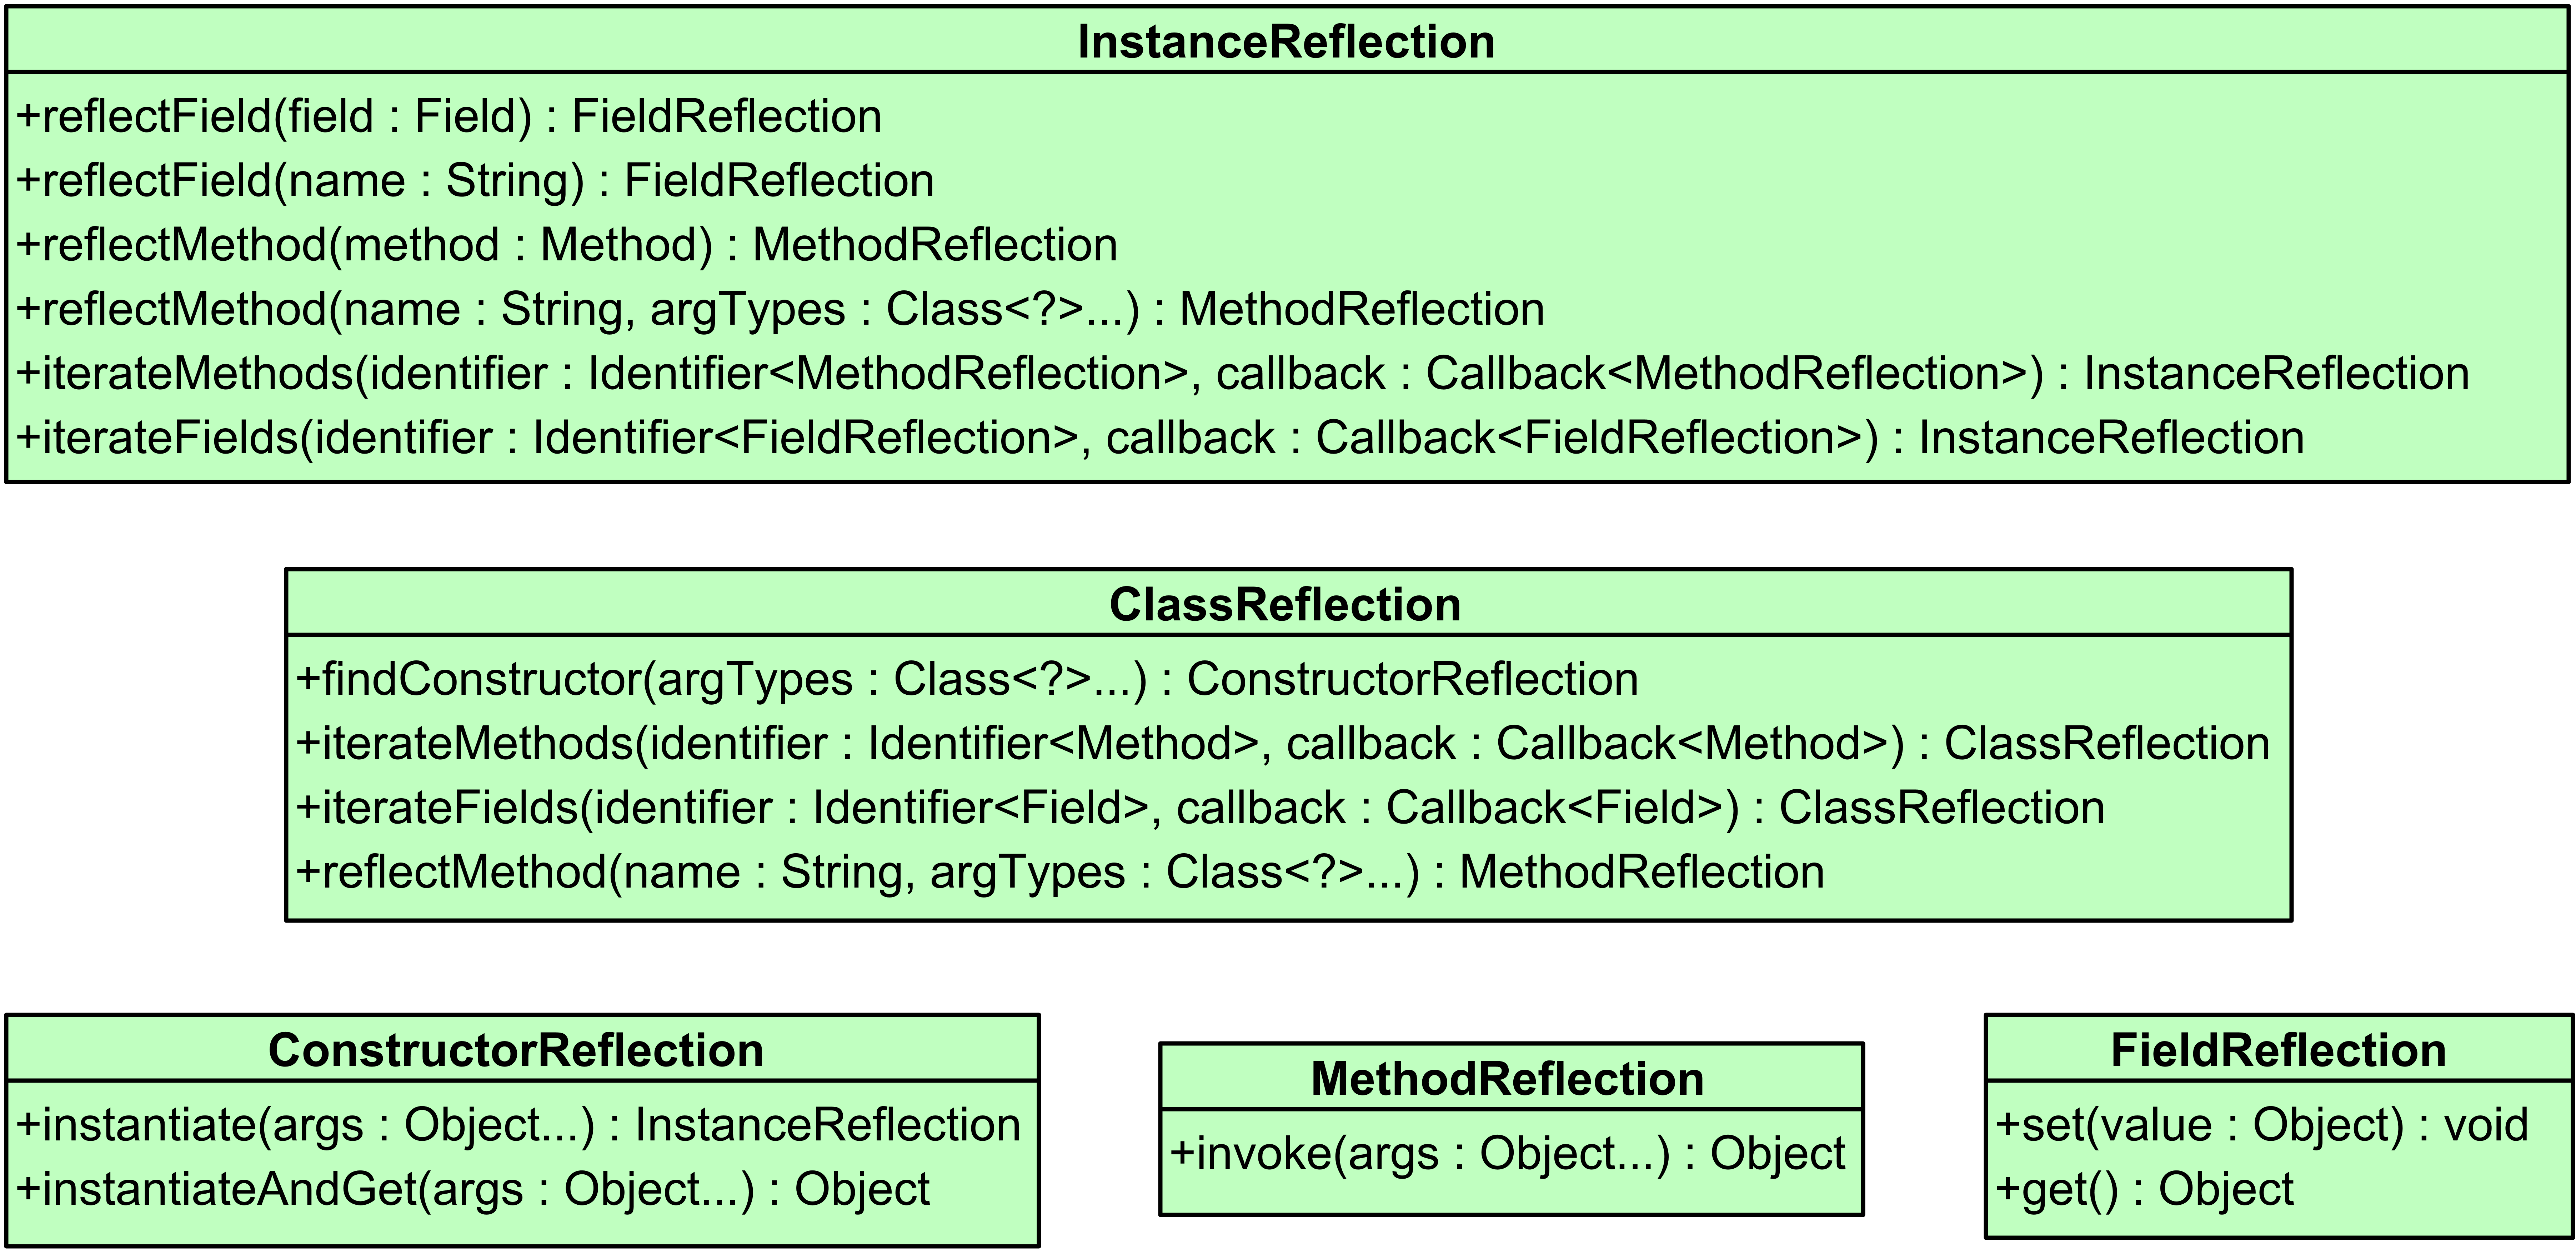
\includegraphics[width=\textwidth]{Abbildungen/ReflectionScopes.png}
	\caption{Diagramm -- \texttt{ReflectionScopes}}
	\label{fig:reflection_scopes}
\end{figure}
\noindent Aus den Klassendiagrammen ist schlusszufolgern, dass alle häufig genutzten reflektiven Operationen durch die Verwendung von Method Chaining, also der Hintereinanderausführung von Methoden, welche Operationen auf dem Objekt ausführen und es dabei zurückgeben, möglich sind. \add{Maybe move to implementation chapter}Ein theoretisches Anwendungsbeispiel der Reflection Schnittstelle ist in \autoref{lst:example_reflection_usage} dargestellt. Dabei wird eine Instanz der \texttt{Test} Klasse mit einem \texttt{Integer} Konstruktorparameter erstellt, welcher als Objektattribut in der Instanz gespeichert wird und mithilfe einer \texttt{InstanceReflection} daraufhin modifiziert wird.
\begin{figure}[H]
	\begin{lstlisting}[caption={Beispiel -- Verwendung der Reflection Schnittstelle.}, captionpos=b, label=lst:example_reflection_usage]
// Klassendefinition
public static class Test {

	private int test;

	public Test(int test) {
		this.test = test;
	}

}
// Instanziierung und Feldzugriff
InstanceReflection i = Reflection.reflect(Test.class)
		.findConstructor(int.class).instantiate(10);
FieldReflection f = i.reflectField("test").forceAccess();
f.set(42);
System.out.println(f.get()); // 42
	\end{lstlisting}
\end{figure}
\subsubsection{Schnittstelle: Klassenpfad}
Damit die Automatisierungsmaßnahmen nach \autoref{freq1} und \autoref{freq5} zum Finden von speziell annotierten Elementen möglich sind, muss eine Art von Klassenpfad-Scanner implementiert werden. Dabei werden alle Klassen, welche in den durch \texttt{Classloader} Instanzen bereitgestellten Klassenpfaden gefunden werden, nach den jeweiligen Annotationen gefiltert (siehe \autoref{fig:classpath_scanprocess}). Das Finden aller Klassen im Klassenpfad muss sowohl für normale Dateisysteme als auch für Applikationen, welche in Java Archiven gepackt worden sind, möglich sein. Um Klassen auf beispielsweise Annotationen zu filtern darf, aufgrund von möglichen Sicherheitsrisiken und Performanceproblemen, kein \texttt{Class} Objekt mittels \texttt{Class\#forName} erstellt werden. Dadurch soll verhindert werden, dass eventuelle \texttt{static}-Blöcke ausgeführt werden. Das Scannen einer Klasse, ohne den \texttt{static}-Block auszuführen, kann durch die ASM Bibliothek\footref{ft:asm}, mithilfe des Besucher Entwurfsmusters erfolgen. Außerdem muss der Scanprozess eine gewisse Konfigurierbarkeit aufweisen, da manuell \texttt{Classloader} Instanzen zum Scanprozess hinzugefügt werden sollen und um eine optimale Performance zu gewährleisten, soll ein initialer Paketname oder Teilstring eines Paketes angegeben werden können, damit nicht benötigte Klassen, schon im Scanprozess ignoriert werden. Ergebnisse des Scans müssen in einem Cache zwischengespeichert werden, damit nicht jeder Filtervorgang den Klassenpfad erneut scannen muss und somit unnötigerweise einen Performance-Hotspot kreiert.
\begin{figure}[H]
	\centering
	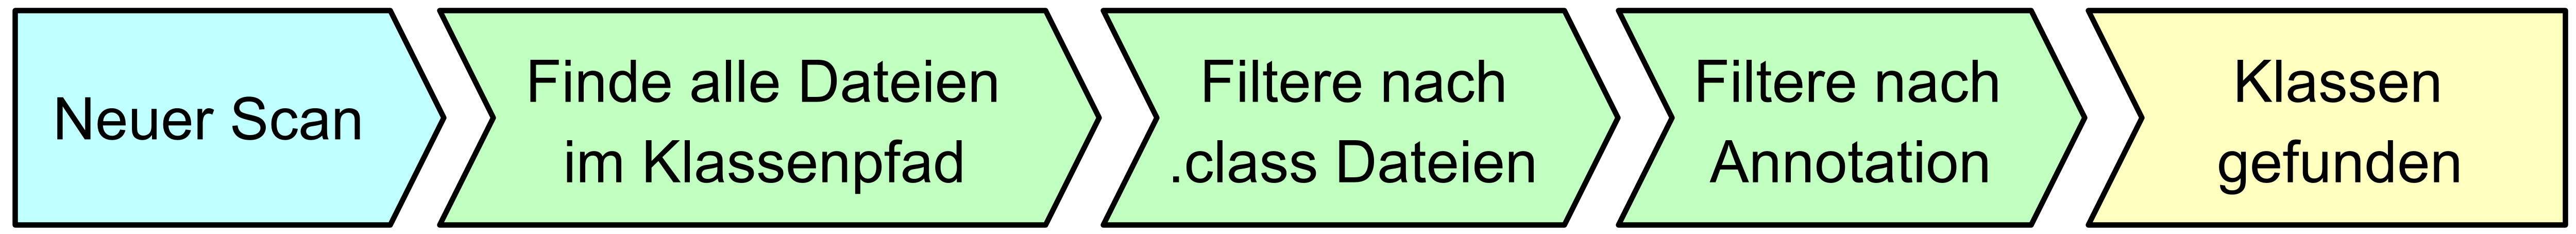
\includegraphics[width=\textwidth]{Abbildungen/Klassenpfad Scanprozess.png}
	\caption{Diagramm -- Klassenpfad-Scanprozess.}
	\label{fig:classpath_scanprocess}
\end{figure}
\subsubsection{Schnittstelle: Lokalisierung}